\documentclass[12pt]{article}
\usepackage{amsmath}
\usepackage{graphicx}
\usepackage{hyperref}
\usepackage{listings}
\usepackage{color}

\title{Operating System Course Report - First Half of the Semester}
\author{A class}
\date{\today}

\begin{document}

\maketitle
\newpage

\tableofcontents
\newpage

\section{Introduction}
This report summarizes the topics covered during the first half of the Operating System course. It includes theoretical concepts, practical implementations, and assignments. The course focuses on the fundamentals of operating systems, including system architecture, process management, CPU scheduling, and deadlock handling.

\section{Course Overview}
\subsection{Objectives}
The main objectives of this course are:
\begin{itemize}
    \item To understand the basic components and architecture of a computer system.
    \item To learn process management, scheduling, and inter-process communication.
    \item To explore file systems, input/output management, and virtualization.
    \item To study the prevention and handling of deadlocks in operating systems.
\end{itemize}

\subsection{Course Structure}
The course is divided into two halves. This report focuses on the first half, which covers:
\begin{itemize}
    \item Basic Concepts and Components of Computer Systems
    \item System Performance and Metrics
    \item System Architecture of Computer Systems
    \item Process Description and Control
    \item Scheduling Algorithms
    \item Process Creation and Termination
    \item Introduction to Threads
    \item File Systems
    \item Input and Output Management
    \item Deadlock Introduction and Prevention
    \item User Interface Management
    \item Virtualization in Operating Systems
\end{itemize}

\section{Topics Covered}

\subsection{Basic Concepts and Components of Computer Systems}
This section explains the fundamental components that make up a computer system, including the CPU, memory, storage, and input/output devices.

\subsection{System Performance and Metrics}
This section introduces various system performance metrics used to measure the efficiency of a computer system, including throughput, response time, and utilization.

\subsection{System Architecture of Computer Systems}
Describes the architecture of modern computer systems, focusing on the interaction between hardware and the operating system.

\subsection{Process Description and Control}
Processes are a central concept in operating systems. This section covers:
\begin{itemize}
    \item Process states and state transitions
    \item Process control block (PCB)
    \item Context switching
\end{itemize}

\subsection{Scheduling Algorithms}
This section covers:
\begin{itemize}
    \item First-Come, First-Served (FCFS)
    \item Shortest Job Next (SJN)
    \item Round Robin (RR)
\end{itemize}
It explains how these algorithms are used to allocate CPU time to processes.

\subsection{Process Creation and Termination}
Details how processes are created and terminated by the operating system, including:
\begin{itemize}
    \item Process spawning
    \item Process termination conditions
\end{itemize}

\subsection{Introduction to Threads}
This section introduces the concept of threads and their relation to processes, covering:
\begin{itemize}
    \item Konsep Threads
    \item Hubungan antara Threads dan Proses
    \item Manfaat Penggunaan Threads
    \item Multithreading
    \item Threads vs Process
    \item Model Multithreading
    \item Pengelolaan Threads
    \item Penerapan Threads pada Sistem Operasi
\end{itemize}
\subsubsection{Konsep Threads}
Dalam sistem operasi, \textit{thread} merupakan unit terkecil dari eksekusi yang dapat dijadwalkan oleh sistem. Setiap proses di dalam sistem operasi setidaknya memiliki satu \textit{thread} utama, yang disebut \textit{main thread}, tetapi seringkali kita ingin menjalankan beberapa tugas secara paralel dalam satu proses. Di sinilah \textit{thread} tambahan digunakan.

Setiap \textit{thread} memiliki tugas eksekusi sendiri, namun tetap berbagi sumber daya yang sama dengan \textit{thread} lain dalam proses yang sama, seperti memori dan file yang terbuka. Hal ini memungkinkan eksekusi yang lebih efisien dan responsif, terutama dalam aplikasi \textit{multithreading} yang memerlukan penanganan beberapa tugas secara bersamaan. Contoh aplikasinya adalah pada \textit{web server}, di mana \textit{thread-thread} yang berbeda bisa melayani beberapa klien secara bersamaan tanpa mengganggu satu sama lain.

\begin{figure}[h]
    \centering
    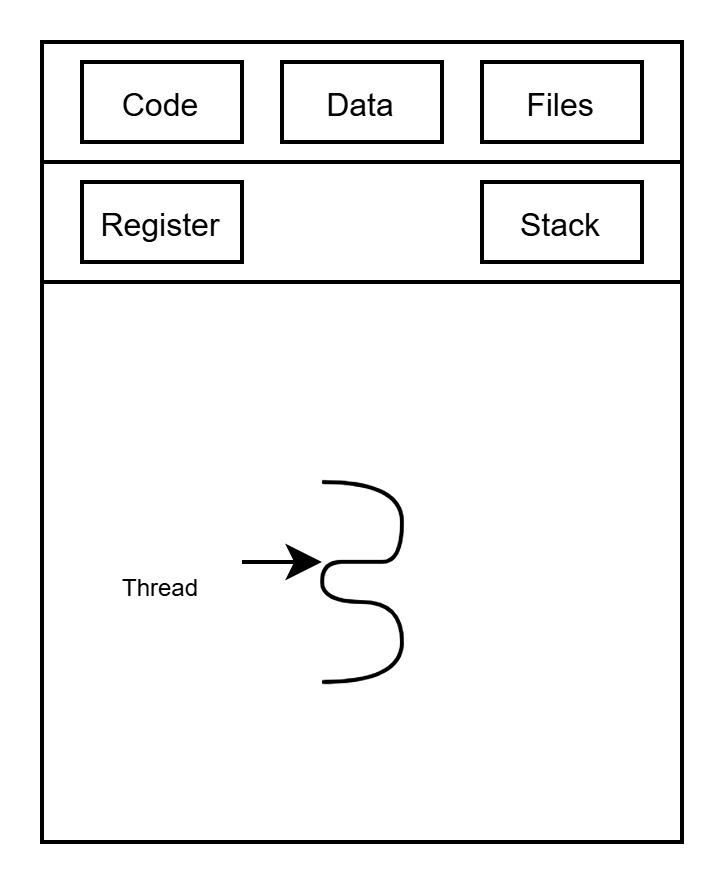
\includegraphics[width=0.5\textwidth]{asset/Gambar-konsep-threads.jpeg}
    \caption{Ilustrasi Konsep \textit{Threads (Single-threaded proses)} }
    \label{fig:konsep-threads}
\end{figure}

Dalam ilustrasi di atas, kita dapat melihat bagaimana beberapa \textit{thread} berjalan secara paralel di dalam satu proses. Setiap \textit{thread} bekerja pada tugas yang berbeda, tetapi tetap menggunakan sumber daya yang sama, seperti memori atau file yang sedang diakses.

Manfaat utama dari penggunaan \textit{threads} adalah kemampuan untuk melakukan beberapa pekerjaan dalam satu proses secara bersamaan, sehingga mempercepat eksekusi program, terutama pada sistem dengan prosesor multiprosesor atau \textit{multicore}.


Stallings, W. (2018). \textit{Operating systems: Internals and design principles} (9th ed.). Pearson Education.
\subsubsection{Hubungan antara Threads dan Proses}
\subsubsection{Manfaat Penggunaan Threads}
\subsubsection{Multithreading}
\subsubsection{Threads vs Process}
\subsubsection{Model Multithreading}
\subsubsection{Pengelolaan Threads}
\subsubsection{Penerapan Threads pada Sistem Operasi}


\subsection{File Systems}
File systems provide a way for the operating system to store, retrieve, and manage data. This section explains:
\begin{itemize}
    \item File system structure
    \item File access methods
    \item Directory management
\end{itemize}

\subsection{Input and Output Management}
Input and output management is key for handling the interaction between the system and external devices. This section includes:
\begin{itemize}
    \item Device drivers
    \item I/O scheduling
\end{itemize}

\subsection{Deadlock Introduction and Prevention}
Explores the concept of deadlocks and methods for preventing them:
\begin{itemize}
    \item Deadlock conditions
    \item Deadlock prevention techniques
\end{itemize}

\subsection{User Interface Management}
This section discusses the role of the operating system in managing the user interface. Topics covered include:
\begin{itemize}
    \item Graphical User Interface (GUI)
    \item Command-Line Interface (CLI)
    \item Interaction between the user and the operating system
\end{itemize}

\subsection{Virtualization in Operating Systems}
Virtualization allows multiple operating systems to run concurrently on a single physical machine. This section explores:
\begin{itemize}
    \item Concept of virtualization
    \item Hypervisors and their types
    \item Benefits of virtualization in modern computing
\end{itemize}

\section{Assignments and Practical Work}
\subsection{Assignment 1: Process Scheduling}
Students were tasked with implementing various process scheduling algorithms (e.g., FCFS, SJN, and RR) and comparing their performance under different conditions.

\subsection{Assignment 2: Deadlock Handling}
In this assignment, students were asked to simulate different deadlock scenarios and explore various prevention methods.

\subsection{Assignment 3: Multithreading and Amdahl's Law}
This assignment involved designing a multithreading scenario to solve a computationally intensive problem. Students then applied **Amdahl's Law** to calculate the theoretical speedup of the program as the number of threads increased.

\subsection{Assignment 4: Simple Command-Line Interface (CLI) for User Interface Management}
Students were tasked with creating a simple **CLI** for user interface management. The CLI should support basic commands such as file manipulation (creating, listing, and deleting files), process management, and system status reporting.

\subsection{Assignment 5: File System Access}
In this assignment, students implemented file system access routines, including:
\begin{itemize}
    \item File creation and deletion
    \item Reading from and writing to files
    \item Navigating directories and managing file permissions
\end{itemize}

\section{Conclusion}
The first half of the course introduced core operating system concepts, including process management, scheduling, multithreading, and file system access. These topics provided a foundation for more advanced topics to be covered in the second half of the course.

\end{document}